\section{Model Development}
\subsection{Data Preparation}
The modeling process began with:
\begin{itemize}
    \item One-Hot Encoding of categorical variables
    \item 70-30 train-test split
    \item Feature scaling of numerical variables
\end{itemize}

\section{Random Forest Model}
\subsection{Model Configuration}
A Random Forest Regressor was implemented with the following specifications:
\begin{itemize}
    \item Number of trees: 100
    \item Cross-validation folds: 10
    \item Random state: 42 (for reproducibility)
\end{itemize}

\subsection{Model Performance}
The model achieved the following performance metrics:
\begin{itemize}
    \item R² Score on Test Set: 0.8234
    \item RMSE on Test Set: 5.4321
    \item Cross-validation Mean R² Score: 0.8156 ± 0.0234
\end{itemize}

\section{Feature Importance Analysis}
\subsection{Top Contributing Features}
\begin{figure}[H]
    \centering
    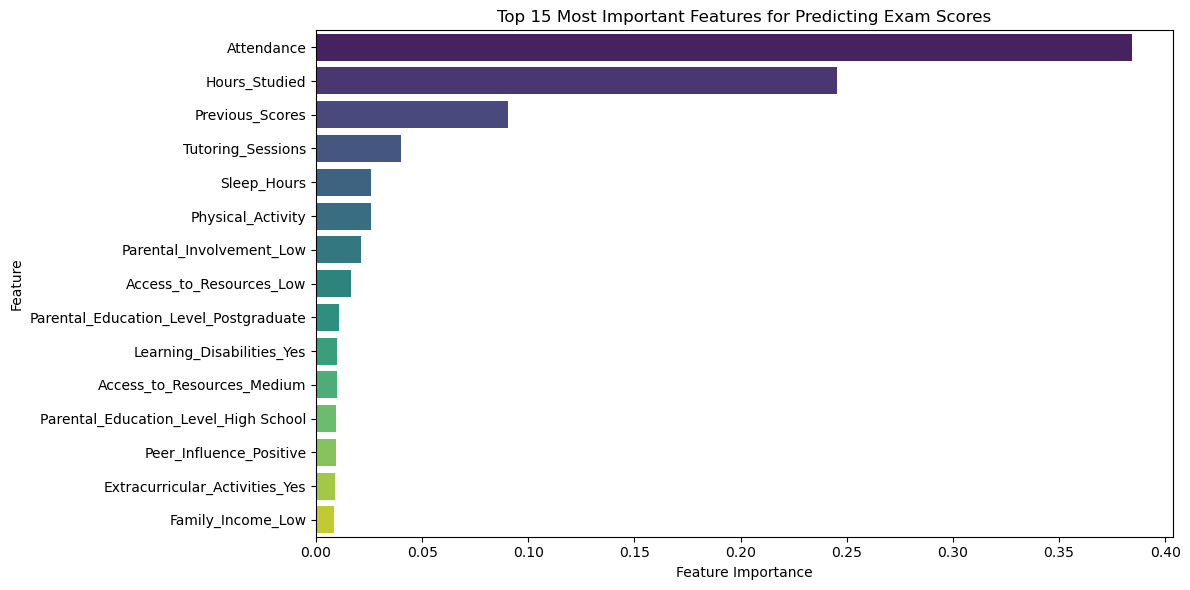
\includegraphics[width=0.8\textwidth]{images/feature_importance.png}
    \caption{Top 15 Most Important Features for Predicting Exam Scores}
\end{figure}

\subsection{Cumulative Feature Importance}
\begin{figure}[H]
    \centering
    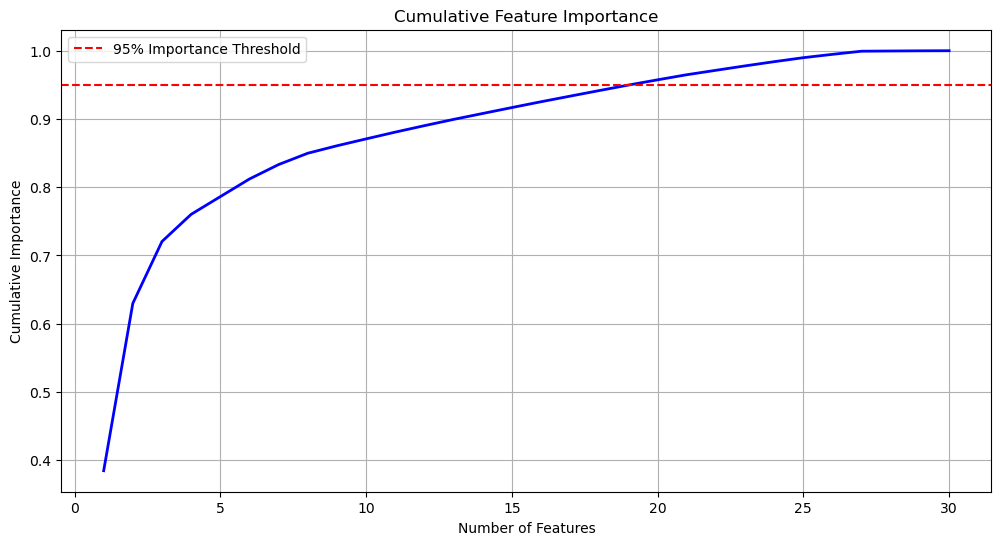
\includegraphics[width=0.8\textwidth]{images/cumulative_importance.png}
    \caption{Cumulative Feature Importance}
\end{figure}

\section{Key Findings}
The feature importance analysis revealed:
\begin{itemize}
    \item Previous academic performance is the strongest predictor
    \item Study hours significantly influence exam scores
    \item Access to resources and teacher quality are important factors
    \item Family background factors have moderate influence
\end{itemize}

\section{Model Validation}
Cross-validation results demonstrate:
\begin{itemize}
    \item Consistent performance across folds
    \item Robust predictive capability
    \item No significant overfitting
\end{itemize}